\section{Modes}

\subsection{Question Types}
SeQG has \textbf{six question types implemented}, enhancing the user's gamified experience with a dynamic, entertaining
app. Each of these question types has been implemented with visual animations depending on the correctness of
the answer and each one of them has an explanation generated by the LLM in case the user answered incorrectly.
The six question types are:
\begin{itemize}
    \item \textbf{Single choice} 
    \item \textbf{Multiple choice} 
    \item \textbf{Think event} 
    \item \textbf{Drag \& drop}
    \item \textbf{Sorting}
    \item \textbf{Line-connect}
\end{itemize}

\subsubsection{Single choice}
In this question type, the user is offered \textbf{two possible solutions} and has to select the correct answer. Once they
touch on the desired answer, the correct answer will be highighted in green. If they have failed, an instant LLM explanation
will be fetched on the same screen for the user to learn:
\begin{figure}[htbp]
    \centering
    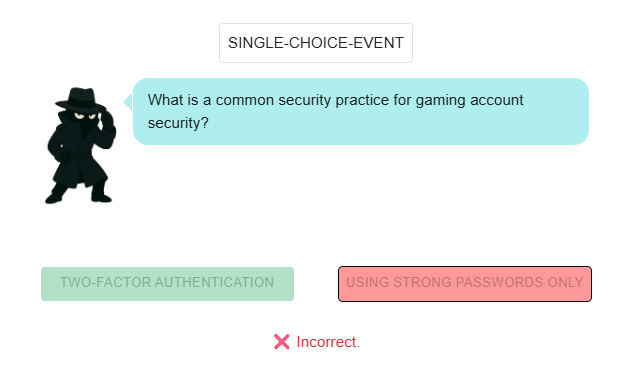
\includegraphics[width=0.6\textwidth]{images/Single_Choice.png}
\end{figure}

\subsubsection{Multiple choice}
Here the user is given \textbf{between two and four possible solutions} and has to select \textbf{all} correct answers. Once every
correct asnwer is selected, the must press the submit button:
\begin{figure}[htbp]
    \centering
    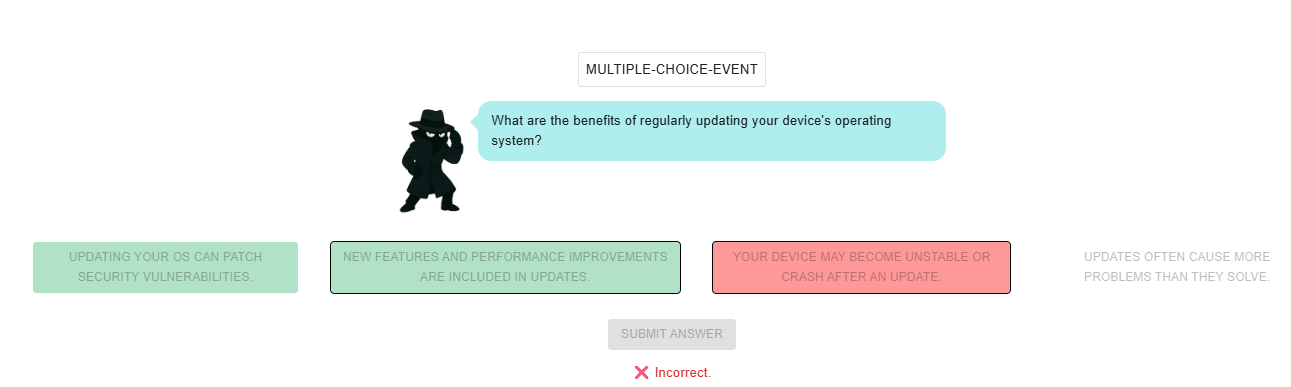
\includegraphics[width=1\textwidth]{images/Multiple_Choice.png}
\end{figure}

\subsubsection{Think Event}
In the think event, the user must think about the possible answer to the question formulated for \textbf{fifteen seconds}. Once the
time is up, they must (honestly) select whether they knew the correct answer or not:
\begin{figure}[htbp]
    \centering
    \begin{minipage}[t]{0.49\textwidth}
        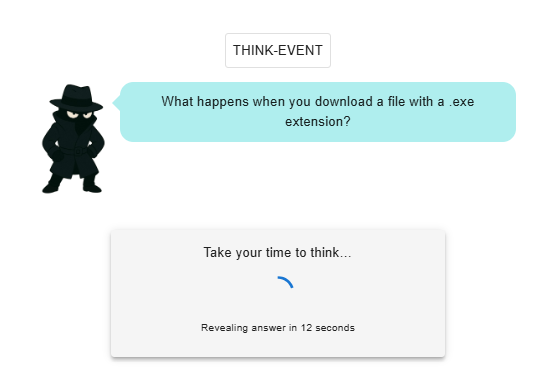
\includegraphics[width=\textwidth]{images/Think_Event.png}
    \end{minipage}
    \hfill
    \begin{minipage}[t]{0.49\textwidth}
        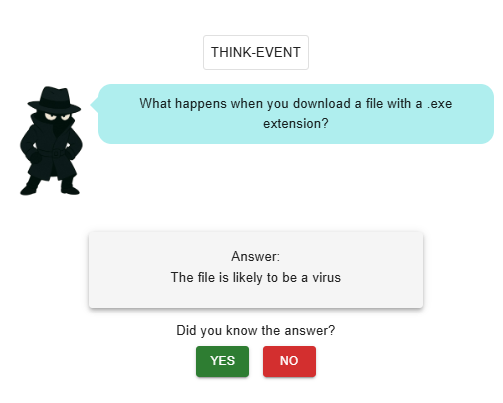
\includegraphics[width=\textwidth]{images/Think_Event_2.png}
    \end{minipage}
\end{figure}

\subsubsection{Drag \& Drop}
The user must drag the boxes into the \textbf{correct category}. There is also the possibility to revert the answer:
\begin{figure}[htbp]
    \centering
    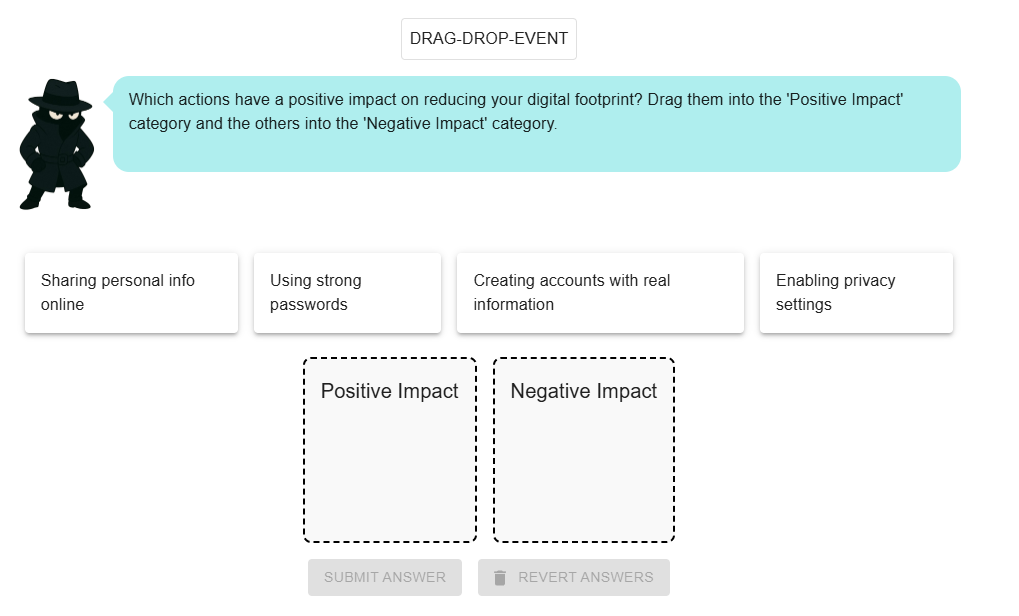
\includegraphics[width=0.8\textwidth]{images/Drag_and_Drop.png}
\end{figure}

\subsubsection{Sorting}
All the answers must be \textbf{correctly sorted}. As before, the user can return to the original order whenever they want:
\begin{figure}[htbp]
    \centering
    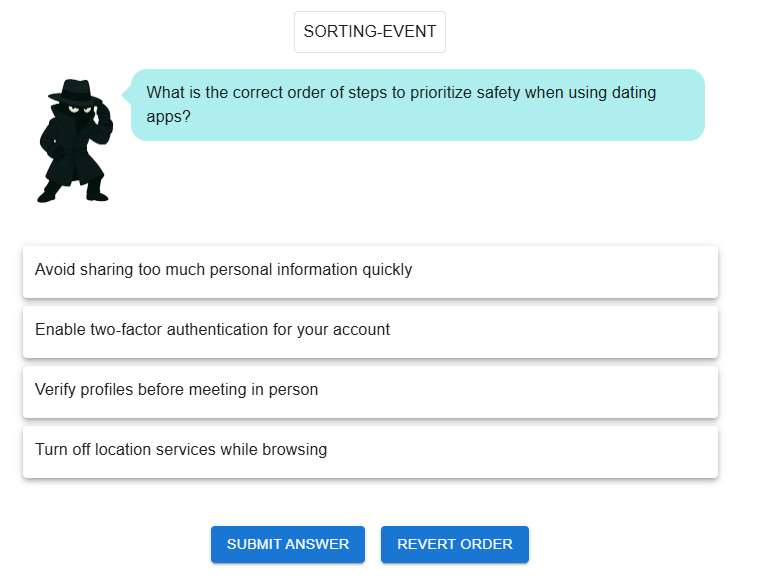
\includegraphics[width=0.6\textwidth]{images/Sorting.png}
\end{figure}

\subsubsection{Line-connect}
In tis question type \textbf{an even number} of boxes is displayed, having to match each item on one side to their correspondant
on the other side. There is also the answer reversal button to start again:
\begin{figure}[htbp]
    \centering
    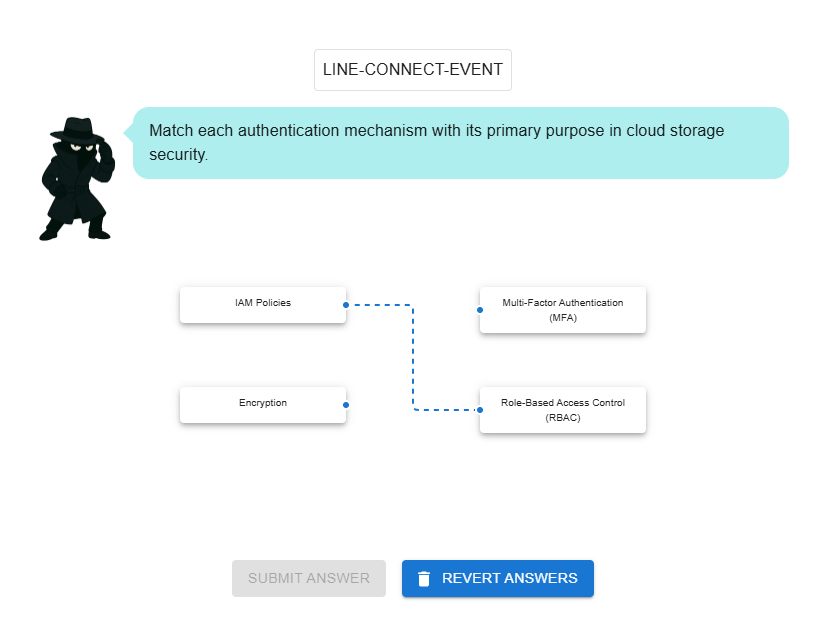
\includegraphics[width=0.8\textwidth]{images/Line_Connect.png}
\end{figure}

\subsection{Gradings}

\begin{figure}[H]
    \centering
    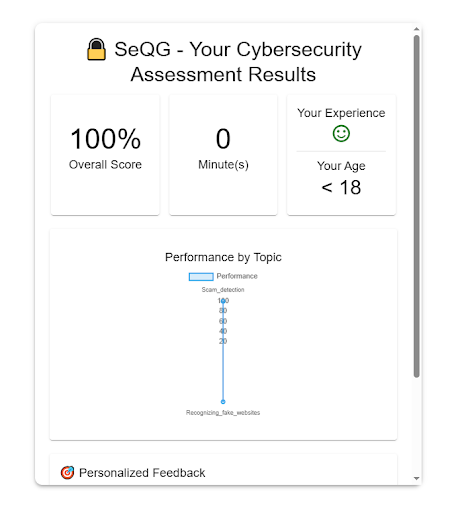
\includegraphics[width=0.4\textwidth]{images/Grading2.png}
    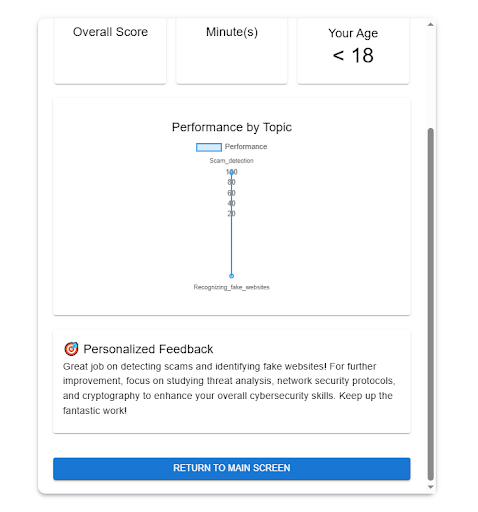
\includegraphics[width=0.4\textwidth]{images/Grading3.png}
    \caption{Dashboard}
\end{figure}
When the user finishes their session (in both guest and private modes), a dashboard appears summarizing their performance. 
To enhance user feedback and engagement in SeQG, the dashboard includes radar charts assessing the user's performance 
across each specific cybersecurity topic, generated with Chart.js. The diagram is split into two if there are more 
than eight topics, to avoid exceeding the visual limit. The dashboard also includes personalized feedback, as 
shown in Figure 2.5, which highlights the user's strengths and weaker areas during their session, encouraging 
them to use SeQG again to improve their cybersecurity awareness. User Progress is persistently stored in a 
structured JSON format if the user started a private session, including metadata such as their userID, age, 
experience and per-topic experience.


\begin{figure}[H]
    \centering
    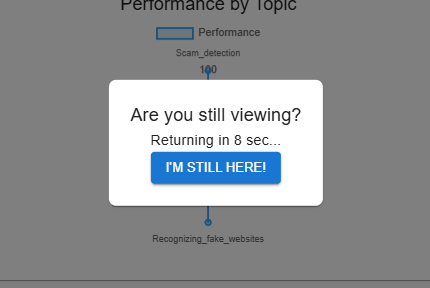
\includegraphics[width=0.35\textwidth]{images/Grading1.png}
    \caption{Inactivity timer pop-up message}
\end{figure}
The interface also includes an inactivity timer that triggers a message in the center of the screen after 60 seconds 
of no interaction. The user then has 10 seconds to confirm their presence; otherwise, the session is closed and the 
system returns to the main screen.